% Options pour le documentclass:
% BCOR : correction d'association
\documentclass[11pt, a4paper, oneside, BCOR=10mm, french]{scrbook}

% Inclus tout les paquets et définie les commandes dans setup.tex

%------------------------------------------------------------------------------
%       package includes
%------------------------------------------------------------------------------
    % font encoding is set up for pdflatex, for other environments see
    % http://tex.stackexchange.com/questions/44694/fontenc-vs-inputenc
    \usepackage[T1]{fontenc}  % 8-bit fonts, improves handling of hyphenations
    \usepackage[utf8x]{inputenc}
    % provides `old' commands for table of contents. Eases the ability to switch
    % between book and scrbook
    \usepackage{scrhack}
    
    
    % ----------------   Page margin   -------------------- %
    \usepackage{geometry}
    \geometry{top=80pt, bottom=80pt}


    % ------------------- layout, default -------------------
    % adjust the style of float's captions, separated from text to improve readabilty
    \usepackage[labelfont=bf, labelsep=colon, format=hang, textfont=singlespacing]{caption}
    \usepackage{chngcntr}  % continuous numbering of figures/tables over chapters
    \counterwithout{equation}{chapter}
    \counterwithout{figure}{chapter}
    \counterwithout{table}{chapter}

    % Uncomment the following line if you switch from scrbook to book
    % and comment the setkomafont line
    %\usepackage{titlesec}  % remove "Chapter" from the chapter title
    %\titleformat{\chapter}[hang]{\bfseries\huge}{\thechapter}{2pc}{\huge}
    \setkomafont{chapter}{\normalfont\bfseries\huge}

    \usepackage{setspace}  % Line spacing
    \onehalfspacing
    % \doublespacing  % uncomment for double spacing, e.g. for annotations in correction

    % ------------------- functional, default-------------------
    \usepackage[dvipsnames]{xcolor}  % more colors
    \usepackage{array}  % custom format per column in table - needed on the title page
    \usepackage{graphicx}  % include graphics
    \usepackage{subfig}  % divide figure, e.g. 1(a), 1(b)...
    \usepackage{amsmath}  % |
    \usepackage{amsthm}   % | math, bmatrix etc
    \usepackage{amsfonts} % |
    \usepackage{calc}  % calculate within LaTeX
    \usepackage[unicode=true,bookmarks=true,bookmarksnumbered=true,
                bookmarksopen=true,bookmarksopenlevel=1,breaklinks=false,
                pdfborder={0 0 0},backref=false,colorlinks=false]{hyperref}


    %==========================================
    % You might not need the following packages, I only included them as they
    % are needed for the example floats
    % ------------------- functional, custom -------------------
    \usepackage{bm}  % bold greek variables (boldmath)
    \usepackage{tikz}
    
    \usetikzlibrary{positioning}  % use: above left of, etc

    % Improves general appearance of the text
    \usepackage[protrusion=true,expansion=true, kerning]{microtype}

%------------------------------------------------------------------------------
%       (re)new commands / settings
%------------------------------------------------------------------------------
    % ----------------- referencing ----------------
    \newcommand{\secref}[1]{Section~\ref{#1}}
    \newcommand{\chapref}[1]{Chapter~\ref{#1}}
    \renewcommand{\eqref}[1]{Equation~(\ref{#1})}
    \newcommand{\figref}[1]{Figure~\ref{#1}}
    \newcommand{\tabref}[1]{Table~\ref{#1}}

    % ------------------- colors -------------------
    \definecolor{darkgreen}{rgb}{0.0, 0.5, 0.0}
    % Colors of the Albert Ludwigs University as in
    % https://www.zuv.uni-freiburg.de/service/cd/cd-manual/farbwelt
    \definecolor{UniBlue}{RGB}{0, 74, 153}
    \definecolor{UniRed}{RGB}{193, 0, 42}
    \definecolor{UniGrey}{RGB}{154, 155, 156}


    % ------------------- layout -------------------
    % prevents floating objects from being placed ahead of their section
    \let\mySection\section\renewcommand{\section}{\suppressfloats[t]\mySection}
    \let\mySubSection\subsection\renewcommand{\subsection}{\suppressfloats[t]\mySubSection}


    % ------------------- marker commands -------------------
    % ToDo command
    \newcommand{\todo}[1]{\textbf{\textcolor{red}{(TODO: #1)}}}
    \newcommand{\extend}[1]{\textbf{\textcolor{darkgreen}{(EXTEND: #1)}}}
    % Lighter color to note down quick drafts
    \newcommand{\draft}[1]{\textbf{\textcolor{NavyBlue}{(DRAFT: #1)}}}


    % ------------------- math formatting commands -------------------
    % define vectors to be bold instead of using an arrow
    \renewcommand{\vec}[1]{\mathbf{#1}}
    \newcommand{\mat}[1]{\mathbf{#1}}
    % tag equation with name
    \newcommand{\eqname}[1]{\tag*{#1}}


    % ------------------- pdf settings -------------------
    % ADAPT THIS
    \hypersetup{pdftitle={The great title!},
                pdfauthor={Carrio Florian},
                pdfsubject={Rapport du TER du Jeu de Go},
                pdfkeywords={deep learning, awesome algorithm,  undergraduate thesis},
                pdfpagelayout=OneColumn, pdfnewwindow=true, pdfstartview=XYZ, plainpages=false}


    %==========================================
    % You might not need the following commands, I only included them as they
    % are needed for the example floats

    % ------------------- Tikz styles -------------------
    \tikzset{>=latex}  % arrow style


    % ------------------- algorithm ---------------------
    % Command to align comments in algorithm
    %\newcommand{\alignedComment}[1]{\Comment{\parbox[t]{.35\linewidth}{#1}}}
    % define a foreach command in algorithms
    %\algnewcommand\algorithmicforeach{\textbf{foreach}}
    %\algdef{S}[FOR]{ForEach}[1]{\algorithmicforeach\ #1\ \algorithmicdo}
    \usepackage[english, frenchb]{babel}
    \usepackage[french]{algorithme}


\usepackage[french]{algorithm2e}
\usepackage{algorithm}
\usepackage{algorithmic}
\usepackage[]{amssymb, amsmath}
\usepackage{framed}
\usepackage{natbib}
\usepackage{graphicx}

%%% francisation des algorithmes
\renewcommand{\algorithmicrequire} {\textbf{\textsc{Entrées:}}}
\renewcommand{\algorithmicensure}  {\textbf{\textsc{Sorties:}}}
\renewcommand{\algorithmicwhile}   {\textbf{tantque}}
\renewcommand{\algorithmicdo}      {\textbf{faire}}
\renewcommand{\algorithmicendwhile}{\textbf{fin tantque}}
\renewcommand{\algorithmicend}     {\textbf{fin}}
\renewcommand{\algorithmicif}      {\textbf{si}}
\renewcommand{\algorithmicendif}   {\textbf{finsi}}
\renewcommand{\algorithmicelse}    {\textbf{sinon}}
\renewcommand{\algorithmicthen}    {\textbf{alors}}
\renewcommand{\algorithmicfor}     {\textbf{pour}}
\renewcommand{\algorithmicforall}  {\textbf{pour tout}}
\renewcommand{\algorithmicdo}      {\textbf{faire}}
\renewcommand{\algorithmicendfor}  {\textbf{fin pour}}
\renewcommand{\algorithmicloop}    {\textbf{boucler}}
\renewcommand{\algorithmicendloop} {\textbf{fin boucle}}
\renewcommand{\algorithmicrepeat}  {\textbf{répéter}}
\renewcommand{\algorithmicuntil}   {\textbf{jusqu'à}}

\begin{document}
    % Pas de numéro de page ni quoi que se soit d'ailleurs
    \pagestyle{empty}
    
    % Déscativation des liens hypertexte pour supprimer le warning "destination with same identifier"
    % De fait aucun hyper lien ne peut être mis ici
    \hypersetup{pageanchor=false}
    
    % On inclue la page de garde
    \begin{titlepage}
    \begin{center}
    
    \newcommand{\HorizontalLine}{\rule{\linewidth}{0.3mm}}
    
    {\Large Projet TER de deuxième année de Licence}\\[1.3cm]
    \begin{figure}[h!]
        \centering
        
\includegraphics[scale=1]{figures/experiments/um.png}
        
\includegraphics[scale=0.4]{figures/experiments/fds_logo.jpg}
        \label{fig:logos}
    \end{figure}
    
    % _____________________________________________________________________________
    \HorizontalLine %[0.4cm]
    \begin{spacing}{3}
        {\huge \bfseries Résolveur de problèmes } 
        {\huge \bfseries de vie ou de mort} 
        {\huge \bfseries dans le Jeu de Go}
    \end{spacing}
    \HorizontalLine \\[1.5cm]
    % _____________________________________________________________________________
    
    
    {\huge Aliou Barry Mamadou} \\[0.2cm]
    {\huge Carrio Florian} \\[0.2cm]
    {\huge Huesca Victor} \\[0.2cm]
    {\huge Rodriguez Julien}\\[0.2cm]
    {\huge Soussi Wissem} \\[1cm]
    
    \begin{tabular}[hc]{>{\huge}l >{\huge}l}
      Professeur Encadrant : & Mr.Pompidor Pierre 
    \end{tabular}
    
    \vfill  % move the following text to the bottom
    
    \Large 
    {
        Faculté des Sciences de Montpellier\\
        Département Informatique
        Second Semestre de l'année Universitaire 2016-2017
    }
     
    \end{center}
\end{titlepage}
    
    % Supprime les nom de chapitres du haut et les numéros de page en bas 
    \pagestyle{plain}
    
    % Numéro de page en chiffre romain pour plus de classe ^^
    \frontmatter
    \tableofcontents
    \listoffigures
    %\listoftables
    \listofalgorithms

    % On réactive les hyperliens pour la suite du rapport
    \hypersetup{pageanchor=true}

    \mainmatter
    \chapter{Introduction}\label{chap:introduction}
    \paragraph{}Notre projet a pour but d'élaborer un algorithme capable de trouver, dans plusieurs situations d'une partie de Go si un groupe peut survire ou non. Pour cela nous avons besoin de tout construire depuis zéro, construire la structure de base du jeu, y implémenter les règles pour finir par créer l'algorithme nécessaire à la résolution d'un problème de vie ou de mort.
    
    \section{Présentation du Jeu de Go}
        \subsection{Histoire du Go.}
            \paragraph{}Le Jeu de Go est un jeu de plateau à 2 joueurs né en Chine il y a plusieurs milliers d'années, c'est le plus ancien jeu de stratégie combinatoire abstrait connu actuellement, on raconte qu'il fut créé pendant la période chinoise des Printemps et Automnes.
            
            \paragraph{}Malgré le fait qu'il soit très ancien, le Jeu de Go continue de profiter d'une grande notoriété dans les pays Asiatiques, notamment en Chine, en Corée et au Japon où il a vu naître sa forme actuelle au XVe Siècle pour beaucoup plus récemment s'exporter en Occident où nous l'avons découvert.
            
            \paragraph{}Il a subi ces dernières années une réelle attention de la part des grands de l'informatique notamment Facebook et Google qui se sont battus pendant un longue période pour confectionner une intelligence artificielle capable de battre n'importe quel humain au Go, c'est là que Google DeepMind a réussi avec Alpha Go en 2015 et a ainsi battu le meilleur joueur de Go dans les années 2000 Lee Sedol, sauf à la quatrième parti où celui-ci à vaincu la bête.
            
            \paragraph{}C'est à l'heure actuelle le plus grand rempart jamais franchi dans le domaine du DeepLearning. Cela explique l'engouement actuel autour de l'intelligence artificielle de beaucoup d'entreprises. Réussir ce challenge est alors un tournant symbolique, celui où les ordinateurs surpassent les humains dans une activité que l'on pensait propre à l'humain.
    
        \subsection{Règles du Jeu}
            \paragraph{}Le Jeu de Go se joue à 2 joueurs, chacun d'eux pose à leur tour une pierre d'une couleur distincte sur un plateau quadrillé appelé Goban. Le but est de contrôler le plus vaste territoire, chacun se bat alors avec ses pierres pour envahir le territoire de l'autre tout en protégeant les leur  ! Il est aussi possible de capturer les groupes ennemis, nous faisant alors gagner des points que nous comptabilisons en plus des points rapportés par les territoires que nous possédons. Le gagnant est finalement celui qui obtient le plus de points.


    \section{Méthodologie de travail et environnement technique}
        \subsection{Méthodologie de gestion des versions de codes : GIT}
            \paragraph{}Ayant un module nous dispensant des cours sur cette plate-forme très pratique qu'est GIT, nous avons trouver ça intéressant d'utiliser celle-ci, et pour sûr nous ne l'avons pas regretter ! Chacun peut avancer en équipe et se passer le "témoin" à la manière d'une course de relais sauf que tout le monde peut avancer en même temps sur des points différents ! Malheureusement il y a aussi de légers désagréments, notamment lorsque tout le groupe ne code pas sur la même plate-forme. Cela engendre parfois des problèmes de compatibilité mais au final cela permet aussi une plus grande flexibilité sur le rendu final.
            
            \paragraph{}De plus, lorsque un membre fait des mauvaises modifications sans que nous nous en rendions compte,  et que un peu plus tard tandis que nous buttions sur une erreur, nous réalisons alors que l'erreur venait de là... Heureusement dans sa globalité GIT fut un fabuleux outil que nous utiliserons sans doute pour nos futurs projets. Ainsi que la diversité des système d'exploitation permet aussi d'avoir une portabilité du programme et des débugages différents.
            L'intégralité de notre projet, ses avancées, etc sont disponibles via GIT à l'adresse suivante : \href{https://github.com/Victor333Huesca/Jeu\_de\_Go}{www.github.com/Victor333Huesca/Jeu\_de\_Go}

        \subsection{Choix des technologies}
            \subsubsection{Le C++}
                \paragraph{}Le choix s'est trouvé évident, cela faisait bientôt 2 ans que nous étudions ce langage, plus pour d'autres, d'autant plus que ce soit pour la programmation objet et l'optimisation mémoire celui-ci reste l'un des meilleurs pour exceller sur ces deux plans.
        
            \subsubsection{SFML}
                \paragraph{}La SFML est une bibliothèque originellement destinée au langage C++ mais portée également vers d'autres langages divers et variés. Celle-ci permet -entre autre- un affichage graphique, des outils système, réseau et même audio.\\
                Notre choix s'est porté sur celle-ci car elle est extrêmement bien documentée (en français en plus) et elle présente un bon rapport entre simplicité d'utilisation et possibilités apportées.

        \subsection{Diagramme de tâche prévisionnel Gantt}  
            \paragraph{}Afin de ne pas s'égarer dans le c\oe ur du projet, nous nous sommes réunis pour planifier les étapes clef du projet. Nous nous somme servis de la méthode de Gantt qui est assez intuitive. 
            
            \begin{figure}[h!]
            \centering
            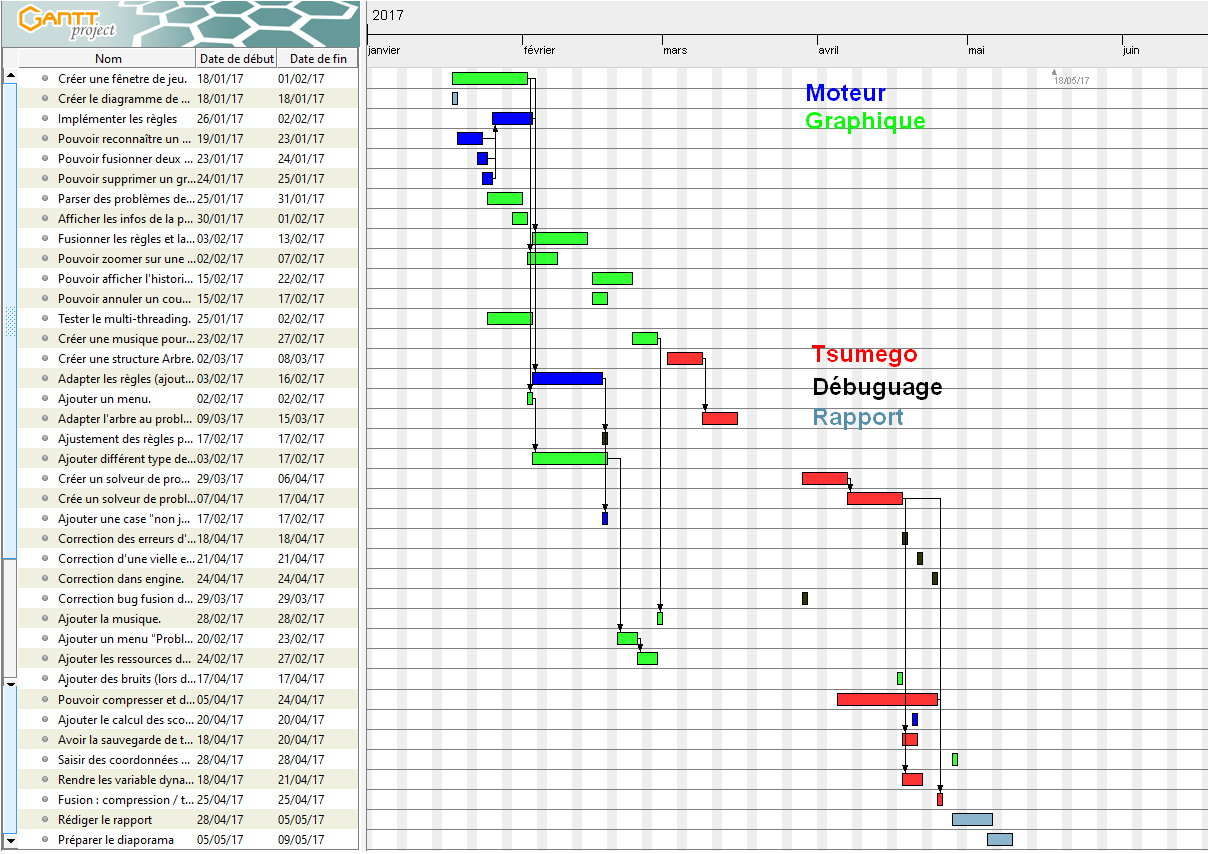
\includegraphics[scale=0.30]{figures/experiments/gantt-previ.png}
            \caption{Gantt Prévisionnel}
            \label{fig:gantt1}
            \end{figure} 
            
            \paragraph{}Évidemment dans un projet certaines parties prennent du retard et -plus rarement- de l'avance. Nous avons tout au long du projet tenu à jour notre planning pour le modifier en conséquence de notre avancement effectif.
            
        \subsubsection{Diagramme final}
            \begin{figure}[h!]
            \centering
            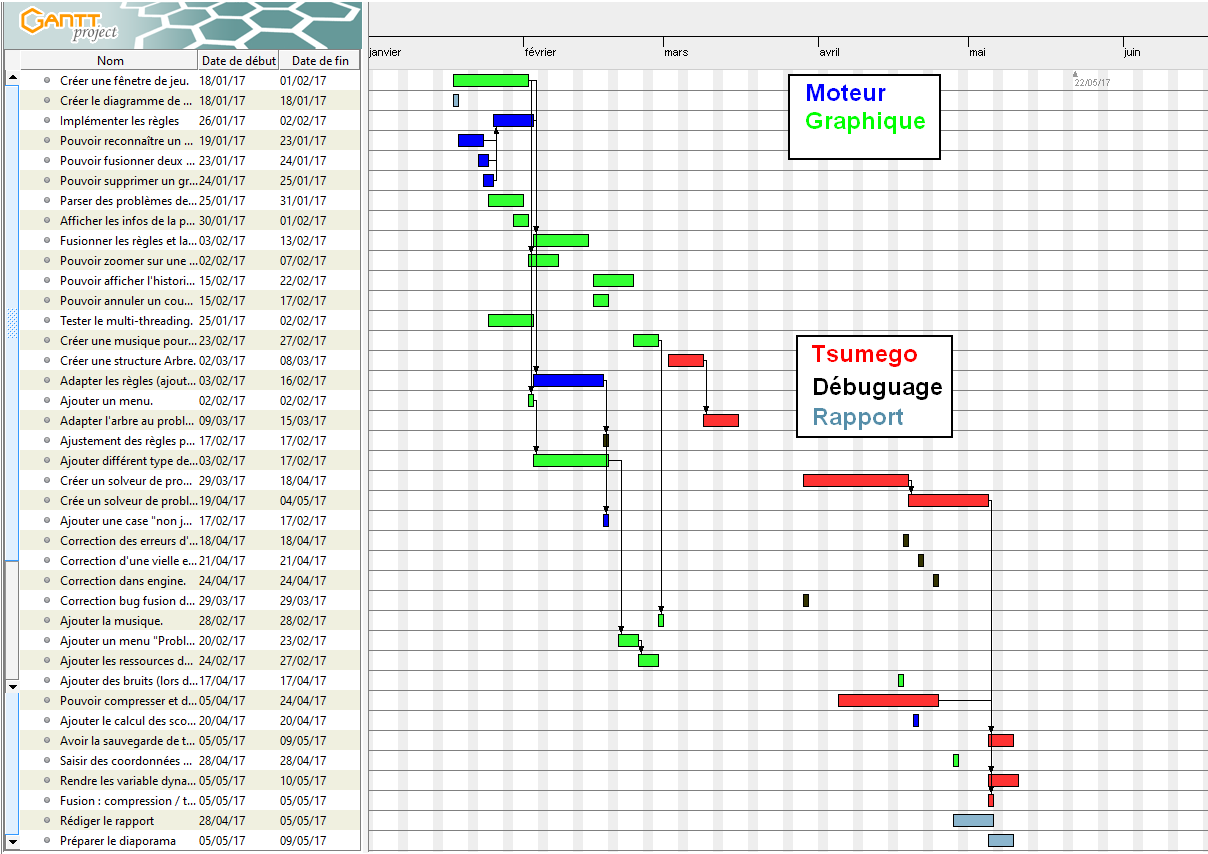
\includegraphics[scale=0.30]{figures/experiments/gantt-final.png}
            \caption{Gantt Final}
            \label{fig:gantt2}
            \end{figure}    

    \chapter{Structures de données et algorithmes de base}\label{chap:moteur}
    Ici nous allons définir les règles du jeu à travers des algorithmes qui permettront d'analyser les situations probables du jeu afin de pouvoir vérifier la légalité des coups joués, ce qui nous rendra apte ensuite à créer l'IA du jeu.
    
    \section{Structure de données}
        \subsection{Goban}
            Pour l'implantation du Goban, nous avons utilisé le paradigme objet du langage C++.\\
            Avec la notion de classe qu'introduit ce dernier, on a pu définir la classe Goban pour manipuler aisément ses données par le biais des fonctions membres.\\ Le Goban se présente comme un plateau de taille 19x19, composé d'état avec ses différentes valeurs.
        \subsubsection{Accès aux états}
            Le goban est en alors un tableau d'états, dont la manipulation à l'aide des accesseurs permettent de  modifié le Goban et simulé le Jeu.
        \subsection{États}
            L'état est une représentation d'une pierre dans le plan, avec ses coordonnées et une valeur qui peut être vide, noir, blanc, KO\_Noir, KO\_Blanc, ou simplement Non jouable (NJ).
        \subsection{Territoires d'un Goban : Les groupes}
            Un Groupe est une liste d'état voisin de même valeur se trouvant dans le Goban.
            
    \section{Algorithmes} 
        \subsection{Algorithme de Recherche}
            La recherche se fait dans le Goban, en deux temps. D'abord on recherche les groupes de couleurs noirs ainsi que les groupes de couleurs blanches. Ensuite on lance la fusion sur chacun des groupes.
            La recherche de Groupe consiste à parcourir tout le Goban en largeur et vérifier si l'état courant appartient à un groupe déjà défini. Le cas échéant on rajoute la pierre à ce groupe et on passe au suivant, autrement on créer un nouveau groupe avec cette pierre.
            
            \begin{algorithme}
                \caption{RechercheGroups}
                \textbf{Données:}
                \Type{val}{VAL} ,
                \Type{Array}{Etat[]}\\
                \textbf{Résultats:} Définir les groupes de la couleur val dans Array\\
                \textbf{Variables:}
                \Type{x, i, j}{entier},
                \Type{groupe}{Groupe}
                %\textbf{Début:}
                
                x $\leftarrow$ 0\\
                \IfThenElse{val = BLANC}
                {val $\leftarrow$ groupsWhite}
                {val $\leftarrow$ groupsBlack}
                \ForFromTo{i}{0}{TGOBAN*TGOBAN}
                {
                    \If{ValArray[i] = val}
                    {
                        j $\leftarrow$ 0 \\
                        \While{j $\leq$ tailleGroups}
                        {
                            \IfThenElse{ ! (Array[i] \in groupe[j])}
                            {
                                \If{groupe[j] doitContenir Array[i]}
                                    {
                                        groupe[j] $\leftarrow$ ajout(Array[i])
                                    }
                            }
                            {
                                j $\leftarrow$ tailleGroups+1
                            }
                            j $\leftarrow$ j + 1
                        }         
                        \If{j = tailleGroups}
                                    {
                                        groupe[i] $\leftarrow$ ajout(Array[i]) 
                                    }
                    }
                }
                
                \caption{Algorithme de recherche groupes}
            \end{algorithme}
    
    \subsection{Algorithme de fusion}
    Pour un ensemble de groupe donnée, cet algorithme vérifie si une pierre d'un groupe est voisin d'une autre  puis rajoute le deuxième groupe au premier et supprime le deuxième sinon il passe au suivant
    
    \begin{algorithme}
       \caption{algorithme de fusion de Groupes}
       \textbf{Données:} 
        \Type{group}{Groupe}\\
        \textbf{Résultat:} Fusionner les groupes de 'group' qui sont voisins\\
        \textbf{Variables:}
             \Type{i, j}{entier} \\
        \textbf{Début:}\\
            \If{tailleGroup > 0}
                        {
                       \ForFromTo{i}{0}{tailleGroup - 1}
                            { \ForFromTo{i}{i+1}{tailleGroup}
                                { \If{groupe[i] estVoisin groupe[j]}
                                    {  groupe[i] fusion groupe[j]\\   supprimer(groupe[j])
                                    }
                                }      
                            }
                        }
    \end{algorithme}
    
    
    \begin{algorithme}
    \caption{Algorithme de recherche et de fusion de groupes}
    \textbf{Données:}
    \Type{goban}{Goban}\\
    \textbf{Résultat:} definir les groupes du goban\\
    \textbf{Début:}\\
    
            rechercheGroups(NOIR, goban.array)\\
            rechercheGroups(BLANC, goban.array)\\
            fusionGroupes(groupesBlack)\\
            fusionGroupes(groupesWhite)
    \end{algorithme}
    
    \subsection{Algorithme de définition des libertés d'un groupe}
    Afin de calculer la liberté d'un groupe il faut d'abord calculer les libertés d'une pierre.
    L'algorithme de liberté s'applique de la façon suivante:
    \begin{itemize}
        \item Pour chaque pierre du groupe faire:
        \begin{itemize}
            \item Vérifier si la pierre se trouve au centre ou dans le bord du goban.
            \item Ajouter les états voisins de la pierre dans un tableau.
        \end{itemize}
        \item Pour la liberté d'un groupe il suffit de voir s'il y a au moins un état dans le tableau des voisins qui est vide, le cas échéant renvoyer vraie sinon faux.\\
    \end{itemize}
    
    \begin{framed}
    Dans l'algorithme il y a les fonctions suivantes:
    \begin{itemize}
    \item \textbf{taille(T)}: Soit un tableau d'éléments \textit{T} la fonction renvoie la taille de \textit{T}.
    \item \textbf{ajoute(e,t)}: Soit un élément \textit{e} et un tableau \textit{t} la fonction ajoute l'élément \textit{e} en queue du \textit{t}.
    \end{itemize}
    \end{framed}
    
    \begin{algorithme}
    \caption{Libertés d'un groupe}
    \textbf{Données :}  
    \Type{gob}{Goban},
    \Type{groupe}{Groupe};\\
    \textbf{Résultat :} renvoie un tableau des libertés du groupe \\
    \textbf{Variables :}
    \Type{l}{entier},\\
    \textbf{Début :}\\
    \For{chaque pierre p de groupe}
    {\For{chaque voisin v de p}
    {\If{v = VIDE}{ajoute(v,l)}}}
    \textbf{renvoyer} l
    \end{algorithme}
    \subsection{Algorithme de captures des groupes}
    A chaque pierre posée il faut vérifier si un ou plusieurs groupes adverses sont tués ou pas et mettre à jour le goban sur lequel se déroule le jeu.\\
    L'algorithme d'élimination est lancé sur les groupes de l'adversaire par rapport à la dernière pierre posée. Pour chaque groupe du tableau des groupes de l'adversaire il faut vérifier différents éléments :\\
    \begin{itemize}
    \item Vérifier que le groupe ait des libertés.
    \item Si le groupe n'a pas de libertés alors  il faudra l'éliminer du goban mais l'éliminer aussi du tableau des groupes.
    \end{itemize}
    \begin{algorithme}
    \caption{Élimination des groupes}
    \textbf{Données :}
    \Type{goban}{Goban},
    \Type{groupes}{Groupe[]};\\
    \textbf{Résultat :} Élimine les groupes sans libertés\\
    \textbf{Variables :}   
    \Type{Libertés}{Etat[]},
    \Type{j}{entier},
    \Type{estLibre}{booléan};\\
    \textbf{Début :}\\
    \For{chaque groupe g de groupes}
    {estLlibre$\leftarrow$0\\
    j$\leftarrow$0\\
    libertés$\leftarrow$libertés(g)\\
    \While{estLibre = faux et j < taille(libertés)}
    {\If{g[j] = VIDE ou g[j] = KO ou g[j] = NJ}
    {estLibre$\leftarrow$vraie\\
    i$\leftarrow$i + 1}
    }
    \If{estLibre = faux}{
    eliminerDuGoban(g,goban)\\
    eliminerDuGroupes(g,Groupes)}
    }
    \end{algorithme}
    \subsection{Algorithme d'élimination des groupes et intégration du KO}
    
    
    A chaque pierre posée il faut vérifier si un ou plusieurs groupes adversaires sont tués puis mettre à jour le goban sur lequel se déroule le jeu.\\
    L'algorithme d'élimination est lancé sur les groupes de l'adversaire par rapport à la dernière pierre posée. Pour chaque groupe du tableau des groupes de l'adversaire il faudra vérifier différents critères :\\
    \begin{itemize}
    \item Vérifier que le groupe ait des libertés.
    \item Si le groupe n'a pas de libertés alors l'éliminer du goban mais l'éliminer aussi du tableau des groupes.
    \end{itemize}
    \begin{algorithme}
    \caption{Élimination des groupes}
    \textbf{Données :}
    \Type{goban}{Goban},
    \Type{groupes}{Groupe[]};\\
    \textbf{Résultat :} Élimine les groupes sans libertés\\
    \textbf{Variables :}   
    \Type{Libertés}{Etat[]},
    \Type{j}{entier},
    \Type{estLibre}{booléan};\\
    \textbf{Début :}\\
    \For{chaque groupe g de groupes}
    {estLlibre$\leftarrow$0\\
    j$\leftarrow$0\\
    libertés$\leftarrow$libertés(g)\\
    \While{estLibre = faux et j < taille(libertés)}
    {\If{g[j] = VIDE ou g[j] = KO ou g[j] = NJ}
    {estLibre$\leftarrow$vraie\\
    i$\leftarrow$i + 1}
    }
    \If{estLibre = faux}{
    eliminerDuGoban(g,goban)\\
    eliminerDuGroupes(g,Groupes)}
    }
    \end{algorithme}
    
    Le KO est un cas particulier qui cause un blocage de la partie il est alors interdit par les règles du jeu.
    Un exemple de KO se trouve dans les figures 1 et 2 , on voit ici que les joueurs peuvent continuer à jouer à l'infini en mangeant les mêmes deux pierres.\\
    Dans la structure de données créer un Etat peut avoir comme valeur \textbf{KOBLANC} qui désigne le KO blanc ou \textbf{KONOIR} qui désigne le KO noir.\\
    \begin{figure}[h!]
    \centering
    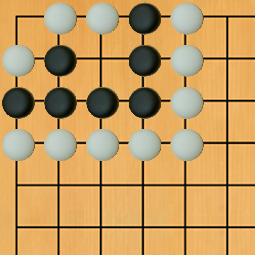
\includegraphics[scale=0.30]{figures/experiments/ko1.png}
    \caption{KO avant}
    \label{fig:button}
        
    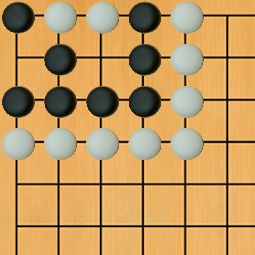
\includegraphics[scale=0.30]{figures/experiments/ko2.png}
    \caption{KO après}
    \label{fig:button}
    \end{figure}
    Un KO retourne vide après un seul coup et une pierre ne peut pas se poser sur un KO de la même couleur sauf si il mange un groupe qui est composé par plus d'une pierre.\\
    Le KO devient, plutôt qu'un algorithme, une intégration de l'algorithme de l'élimination des groupes.\\
                
    \section{Algorithme de définition des gobans fils d'un noeud}
    Pour chaque noeud de l'arbre on calcule tout les coups possibles du joueur et pour chaque coup on créé un goban. On aura de cette manière les gobans fils qui serons créé successivement à la base de ces premiers.\\
    Le nombre de gobans créés sera intuitivement le nombre d'états vides dans le goban de référence.
    Dans l'algorithme il y a les fonctions suivantes:\\
    \begin{itemize}
    \item \textbf{jouer(goban,pierre)}:
    contrôle si par rapport aux règles du jeu on peut poser la pierre dans le goban.\\
    Si le coup est possible alors l'appliquer et renvoyer vraie, sinon faux.
    \item \textbf{ajoute(e,t)}:
    Ajoute l'élément e en queue du tableau t.
    \item \textbf{rechercheGroupes(e,t)}:
    Ajoute l'élément e en queue du tableau t.
    \item \textbf{ajoute(e,t)}:
    Ajoute l'élément e en queue du tableau t.
    \end{itemize}
    
    
    \subsection{Algorithme du suicide}
    Le suicide est un coup avec lequel un joueur peut tuer un ou plusieurs groupe de sa propriété. Ce type de coup est illégal dans le jeu de go, il faudra donc que le programme détecte si un coup du joueur est un suicide ou pas. Pour cela on a créé l'algorithme suivant qui suit les étape suivantes :\\
        \begin{itemize}
            \item Vérifier si l'endroit où on va poser la pierre a des libertés afin de déterminer si c'est un suicide ou pas.
            \item Exécuter le coup sur un deuxième goban virtuel et lancer sur ce dernier la recherche de nouveaux groupes et l'élimination des groupes de l'adversaire relatif à la couleur de la pierre.
            \item Vérifier si le coup a tué un groupe adverse, indiquant alors que c'est pas un suicide.
            \item Enfin lancer sur le goban virtuel l'élimination des groupes de la même couleur que la pierre, puis vérifier si il tue un de ses groupes, prouvant alors le suicide.
        \end{itemize}
        Dans cet algorithme il y a 4 fonctions appelées qui auront les objectifs suivants:\\
        \begin{enumerate}
            \item \textbf{GroupesNoir(Goban)}: Soit une instance de la structure Goban passée en paramètre la fonction renvoie alors ses groupes noirs.
            \item \textbf{GroupesBlanc(Goban)}: Soit une instance de la structure Goban passée en paramètre la fonction renvoie alors ses groupes blancs.
            \item \textbf{PosePierreDansGoban(Pierre,Goban)}: Soit  une pierre et un goban la fonction pose la pierre sur le goban aux coordonnées stockées dans la variable pierre en vérifiant que l'endroit dans le goban soit vide.
            \item \textbf{EliminerGroupes(pierre, goban)}:Soit une pierre et un goban la fonction élimine les groupes sans libertés dans goban avec la même couleur que la pierre. 
            \item \textbf{EliminerGroupesAdversaire(pierre, goban)}:Soit une pierre et un goban la fonction élimine alors les groupes sans libertés dans goban avec la couleur opposée à la pierre initiale. 
        \end{enumerate}
        Il est important de préciser que la fonction de calcule des libertés d'une pierre sera nécessaire aussi.
    
    \begin{algorithme}
    \caption{Est-Suicide?}
    \textbf{Données :}
    \Type{Gob}{Goban},
    \Type{Pierre}{Etat};\\
    \textbf{Résultat :} Renvoie vrai si Pierre cause un suicide dans le Gob, renvoie faux sinon.\\
    \textbf{Variables :}   
    \Type{GroupesAVérifier}{Groupe[]},
    \Type{GroupesAdversaire}{Groupe[]},
    \Type{GroupesAdversaireAprès}{Groupe[]};\\
    \textbf{Début :}\\
     \If{taille(libertés(Pierre)) > 0}{ \textbf{renvoyer} faux}
     goban2 $\leftarrow$ goban\\
     \IfThenElse{Couleur(Pierre) = BLANC}{ GroupesAdversaire $\leftarrow$ groupesNoir(goban2)}{GroupesAdversaire $\leftarrow$ groupesBlanc(goban2)}
     JouerPierreDansGoban(Pierre, goban2)\\
     RechercheGroupes(goban2)\\
     EliminerGroupesAdversaire(Pierre, goban)\\
     \IfThenElse{Couleur(Pierre) = BLANC}{ 
     GroupesAdversaireAprès $\leftarrow$ groupesNoir(goban2)\\
     GroupesAVérifier $\leftarrow$ groupesBlanc(goban2)}
     {GroupesAdversaireAprès $\leftarrow$ groupesBlanc(goban2)\\
     GroupesAVérifier $\leftarrow$ groupesNoir(goban2)}
     \IfThenElse{taille(GroupesAdversaireAprès) < taille(GroupesAdversaire)}
     {\textbf{renvoyer} faux}{
     EliminerGroupes(Pierre, goban)\\
     \If{(Pierre = BLANC et taille(GroupesAVérifier) \neq taille(groupesBlanc(goban2))}{\textbf{renvoyer} vraie}
     \If{(Pierre = NOIR et taille(GroupesAVérifier) \neq taille(groupesNoir(goban2))}{\textbf{renvoyer} vraie}}
     {\textbf{renvoyer} faux}
\end{algorithme}

    \chapter{Interface graphique}\label{chap:GUI}
    \section{Le jeu}
        \subsection{La fenêtre de Jeu}
            \paragraph{}C'est un élément déterminant car il est ce que voit l'utilisateur est c'est par celui-ci est uniquement celui-ci que le programme communique avec ce dernier. Bien que central cet élément \textbf{ne gère pas les choses lui-même}, en effet il se contente de \textbf{communiquer les événements qu'il reçoit} à ses composantes que sont le \textit{Plateau (le Goban)} et \textit{la zone d'infos.}
            
            \paragraph{}La fenêtre de jeu fait donc principalement office \textbf{d'interface} et sa fonction se résume à savoir qui des \textit{infos} ou du \textit{plateau} est apte à \textit{traiter l'information} reçue. C'est donc un des éléments situés au plus \textbf{haut niveau} avec les différents menus, cette catégorie d'objet est celle ayant en charge la \textbf{boucle principale} et s'affichant directement à l'écran.
            
            \begin{figure}[h!]
            \centering
            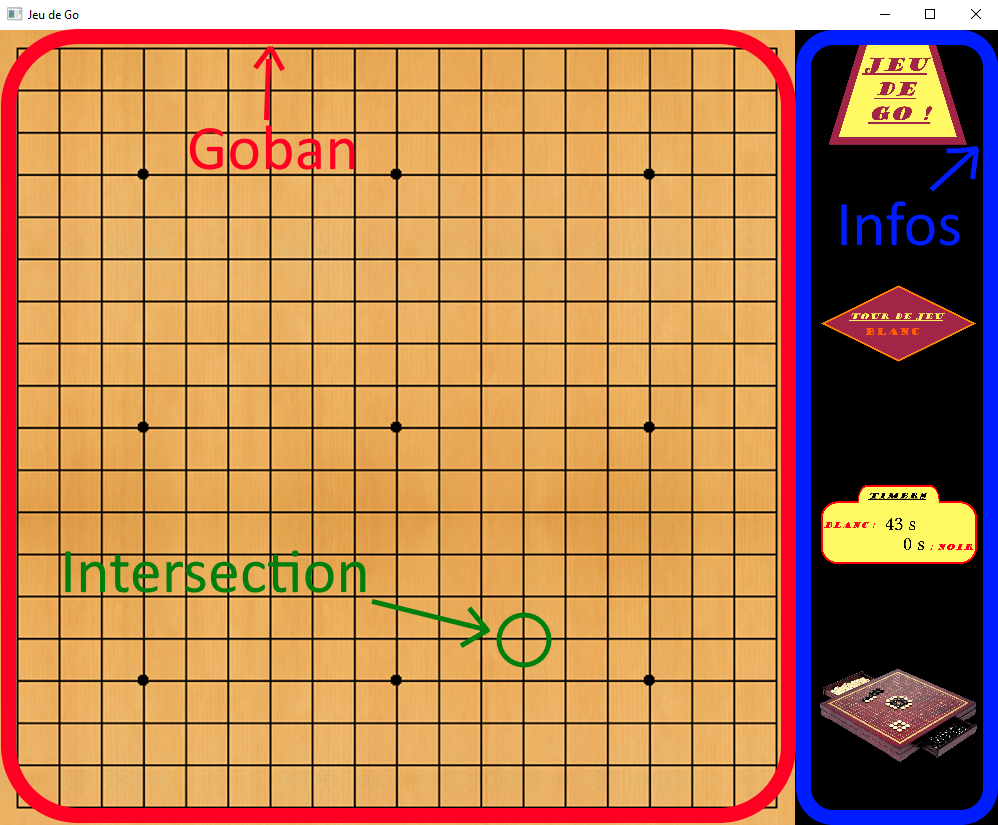
\includegraphics[scale=0.45]{figures/experiments/Fenetre_de_jeu.png}
            \caption{Fenêtre de Jeu}
            \label{fig:game}
            \end{figure}
            
        \subsection{Une partie de Go}
            \paragraph{}Le goban est composé tout d'abord d'un \textbf{visuel} -son apparence- qui peut éventuellement changer selon les goûts de l'utilisateur. On peut aussi souhaiter se concentrer simplement sur une partie du plateau et pour cela il convient d'autoriser un \textbf{zoom} afin de correspondre au mieux à la zone pertinente aux yeux de l'utilisateur.   
            
        	\paragraph{}De plus le plateau est l'élément qui \textbf{interface} avec le \textit{'moteur'} du jeu, c’est à dire les différentes \textit{règles du jeu}. Pour cela il convient de lui permettre de faire la jonction correctement entre le visuel -qui est destiné à l'utilisateur- et ce moteur. Évidemment ceci fonctionne dans les deux sens et \textbf{les actions utilisateur} (clavier, souris, ...) doivent être interceptées par cet élément pour \textbf{être transmises} aux \textit{règles} qui lui dicteront en retour l'action à entreprendre (par exemple pour un feed-back).
        	
        	\paragraph{}Bien qu'il fasse office de passerelle avec le moteur, il convient de ne pas résumer le goban simplement à cette fonction munie d'un visuel. En effet le goban représente avant tout \textbf{la zone de jeu} et celle-ci est composé d'un élément capital : \textit{les intersections} où sont posées les pierres.
        	
    	\subsection{L'intersection}
    	    \paragraph{}Dans un goban l'intersection joue un rôle majeur et chacune d'entre elles possède diverses informations qu'il est nécessaire de bien définir afin de pouvoir les représenter. \\
        	Parmi ces informations on distingue deux types d'information : celles \textbf{propres à chaque intersection} et celles \textbf{communes à toutes les intersections}.      
        	
        	\paragraph{}Pour ce qui est des informations communes, on trouve simplement \textbf{l'apparence des pierres}. Celle-ci doit en effet être la même indépendamment de l'intersection où se trouve la pierre. D'autres informations pourraient être relevées mais elles n'ont pas d'implication dans notre application. C'est notamment le cas du poids des pierres, de leur animation de pose / de prise, de leurs sons dans divers cas, etc...        	
        	
        	\paragraph{}Concernant les informations distinctes, celles-ci sont un peu plus nombreuses. Il faut retenir -entre autres- \textbf{la position} de chaque intersection ainsi que \textbf{sa 'valeur'} (i.e. si c'est une pierre noire, blanche ou s'il n'y a pas de pierre du tout). Pas d'autre information effectivement utilisée n'est à relever ici.
        	
	    \subsection{La zone d'infos}
	        \paragraph{}Si une partie de Go pourrait se résumer à un \textit{plateau et des pierres}, certaines informations manquent cruellement à cette définition. C'est notamment le cas du \textbf{joueur actuel} car le jeu de Go se joue au tour par tour comme la très grande majorité des jeux de plateau. Mais aussi du \textbf{temps passé} par chaque joueur depuis le début de la partie. En effet certaines règles imposent un temps de jeu limité par coup / global ; et lorsque ce n'est pas imposé, il est tout de même souhaitable de disposer visuellement de ces informations.
	         
	         
    \section{Les menus}
        \subsection{Définition des menus}
            \paragraph{}Lorsque l’on développe une \textbf{application graphique} il arrive un moment où il convient d’intégrer un menu à celle-ci afin de la rendre \textbf{navigable et configurable} par l’utilisateur. Malheureusement cette partie peut s’avérer très longue et fastidieuse avant d’arriver à un résultat convenable. Aussi il faut bien souvent choisir entre des menus lourds très personnalisables mais longs à intégrer et des menus plus génériques mais intégrables rapidement. Nous avons opté pour cette seconde méthode qui –bien qu’elle soit plus longue à préparer- permet de \textbf{rajouter facilement des menus, des items, etc…} Nous allons détailler ici les menus génériques tels qui \textit{peuvent être intégrés} à n’importe quel autre programme.
            
            \begin{figure}[h!]
            \centering
            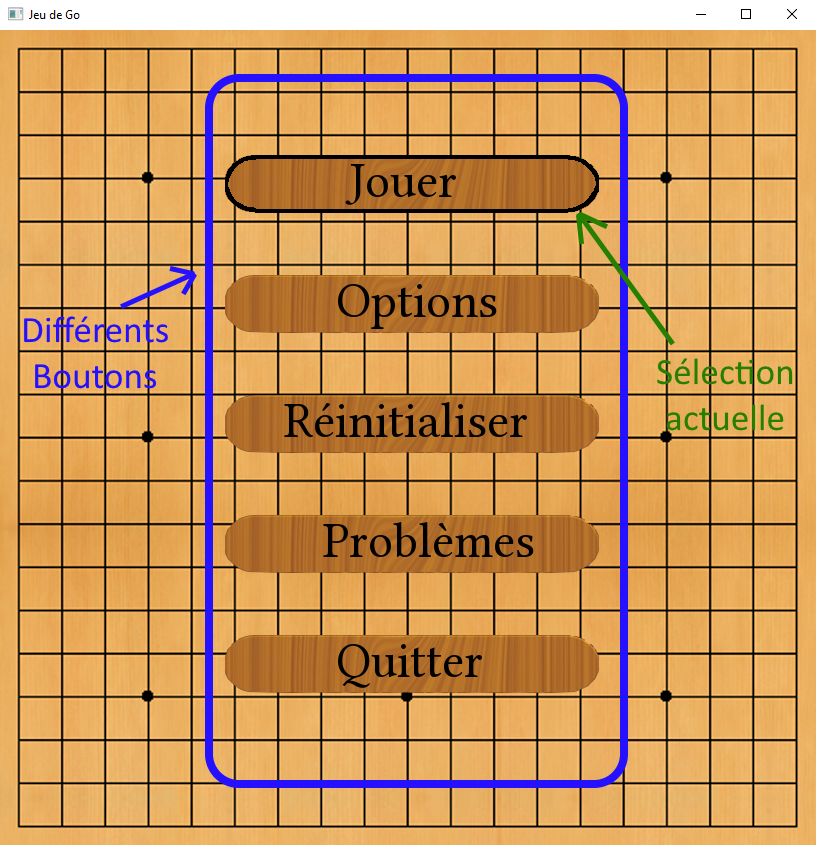
\includegraphics[scale=0.45]{figures/experiments/Menu_main.png}
            \caption{Menu où les boutons ont la même texture mais un texte différent}
            \label{fig:butto_txt}
            \end{figure}
            
	        \paragraph{}Pour cela nous devons identifier ce qu’est un menu et ce qu’il permet de réaliser. Tout d’abord un menu est un \textbf{élément visuel navigable} qui permet à \textit{l’utilisateur} \textbf{d’interagir} avec le programme. Chaque menu est donc composé d’éléments visuels tels que \textbf{l’arrière-plan}. De plus chaque menu possède différents \textit{boutons}. Comme dit ci-dessus les menus doivent être capables d’interagir avec l’utilisateur, notamment un menu doit permettre de \textbf{naviguer} librement entre les différents \textit{choix} qu’il propose ainsi que de mettre en valeur le \textit{choix actuellement sélectionné} par l’utilisateur. En plus de pouvoir naviguer parmi différents choix, l’utilisateur peut souhaiter aussi pouvoir \textbf{valider} le choix actuellement sélectionné, il faut donc lui en donner l’opportunité. 
	        
            \paragraph{}Une fois que ces principes de bases sont posés on peut réfléchir à la façon dont les menus doivent être créés par le programmeur. Pour créer un menu il faut donc \textbf{une position}, éventuellement \textbf{ menu précédent} et \textbf{un aspect} (l’arrière-plan). Le menu ne se suffisant pas à lui-même il faut permettre \textbf{l’ajout \textit{d’items}} en son sein. Nous nous sommes arrêté ici car ces menus doivent répondre à des besoins basiques notre projet étant en temps limité.
             
        \subsection{Définition des items}
            \paragraph{}Comme \textit{un menu} ne peut se passer de boutons nous avons créé ceux-ci et, là aussi, un peu de réflexion a été de mise. Tout comme les menus, les boutons possèdent \textbf{un aspect}. En fait ils en possèdent même plusieurs selon \textbf{leur état}.
            \paragraph{}En effet les boutons possèdent différents états qui peuvent parfois se \textbf{cumuler}. Notamment ils peuvent être \textbf{sélectionnés}, \textbf{survolés} par la souris, \textbf{enfoncés} par un click, voir ne pas avoir d’état particulier, un peu à la manière des \textit{liens HTML}.
            
            \begin{figure}[h!]
            \centering
            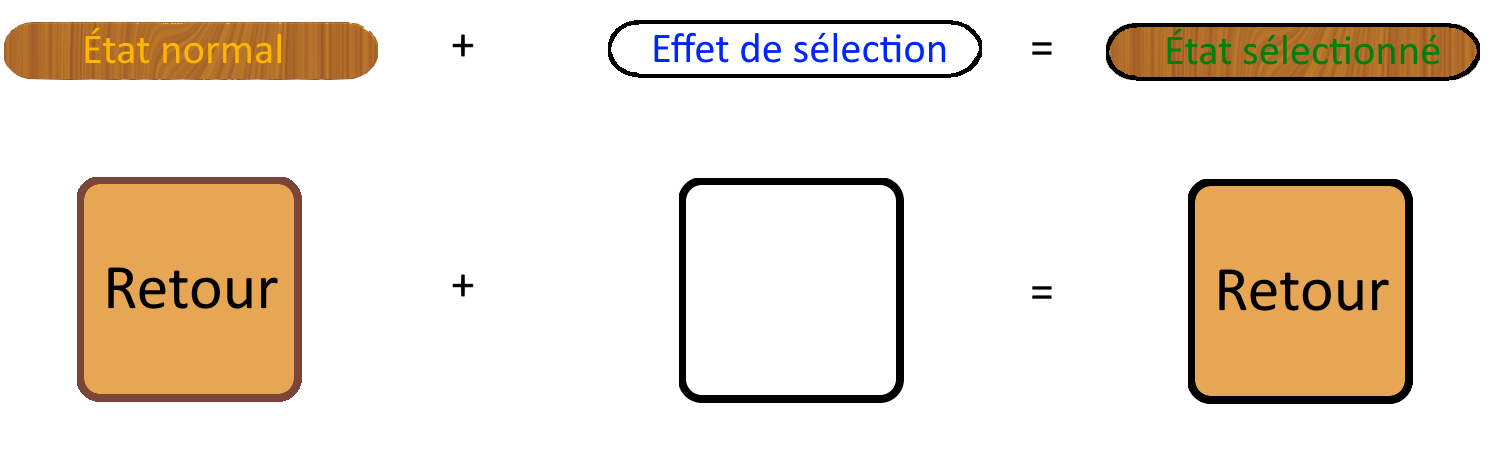
\includegraphics[scale=0.30]{figures/experiments/Effet_Select.png}
            \caption{Application d'effets aux boutons}
            \label{fig:button}
            \end{figure}
            
            \paragraph{}Ces états déterminent donc \textbf{l’affichage du bouton} et c’est pourquoi celui-ci possède \textit{plusieurs aspects} même si un seul est affiché à la fois. Le bouton doit contenir en permanence son \textbf{état actuel} qui sera changé par le \textit{menu auquel il appartient}. Enfin pour en finir avec l’aspect des boutons ceux-ci possèdent bien évidement \textbf{une position} relative au menu auquel ils appartiennent ainsi qu’\textbf{une zone de collision} permettant au \textit{menu} de déterminer si l’utilisateur pointe sa souris sur tel ou tel bouton.
            
            \paragraph{}Enfin les boutons ne sont pas juste là pour décorer et leur fonction principale est de permettre \textbf{d’effectuer une action} lors de la sélection de ceux-ci. Une fois \textit{validé} un bouton peut permettre des actions aussi \textit{diverses} que couper la musique revenir au menu précédent, lancer une partie de Go ou même quitter le jeu.

        \subsection{Les cas spéciaux}
            \paragraph{}Une fois les menus et boutons créés nous nous sommes rendu compte en les utilisant -pour créer les différents menus du jeu- que certaines tâches répétitives persistaient et que les menus pouvaient donc encore être améliorés. 
            
            \begin{figure}[h!]
            \centering
            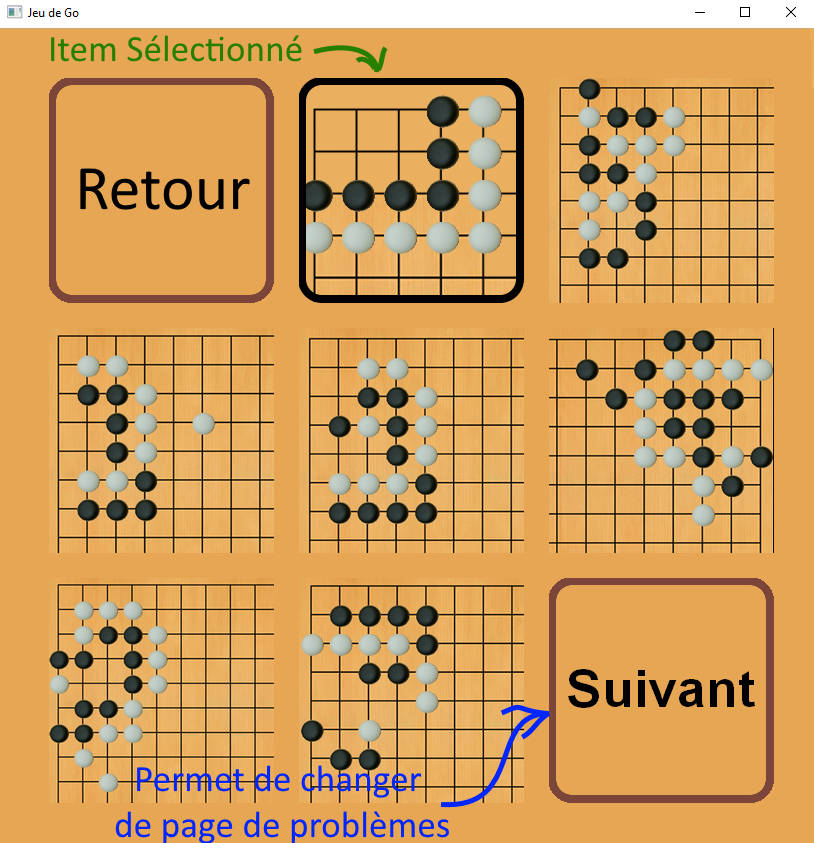
\includegraphics[scale=0.45]{figures/experiments/Menu_pbs.png}
            \caption{Menu où chaque bouton a sa propre texture}
            \label{fig:menu_prbls}
            \end{figure}
            
            \paragraph{}Par exemple dans le cas où \textit{sélectionner un item} ne doit \textbf{pas changer son apparence} mais simplement lui appliquer une \textbf{mise en valeur} (par exemple un lisserait noir l’entourant dans notre cas). Pour régler ceci et afin \textbf{d’alléger la mémoire} dans ce genre de cas de figure assez courant nous avons choisi de dériver notre objet menu en une variante contenant -en plus de tout ce que possède déjà un menu- \textbf{l’effet à appliquer} au bouton sélectionné. 
             
            \paragraph{}Nous avons aussi fait le choix de dériver à nouveau notre menu pour lui ajouter une autre fonctionnalité : \textbf{le texte}. En effet nous souhaitions créer des \textbf{boutons avec un texte} et nous n’avions besoin que d’une \textbf{police de caractère} pour tous les boutons du menu –nul besoin d’alourdir la mémoire avec la même police chargé X fois en mémoire là où une suffirait.
            Pour aller avec ces deux nouveaux menus nous avons de la même manière dérivé les boutons pour qu’ils puissent contenir soit leur \textit{propre texture} pour le $1^{er}$ cas soit \textit{leur texte} pour le $2^{nd}$ cas.
            
            \paragraph{}Tout ceci permet dans cette application un léger \textbf{gain mémoire} (dans notre exemple celui-ci est de d’un facteur 50) qui, dans le cas d’une application plus volumineuse avec de nombreux menus et surtout des ressources plus gourmandes en mémoires, permet d’atteindre des gains bien plus conséquent.
            
            \begin{figure}[h!]
            \centering
            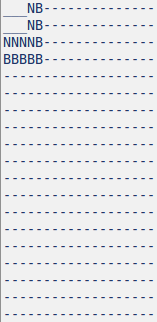
\includegraphics[scale=0.39]{figures/experiments/fichierGo.png}
            \caption{Le fichier .go du problème du 6 en coin}
            \label{fig:menu_prbls}
            \end{figure}

    \section{Les ressources}
        \subsection{La musique}
            \paragraph{}La musique a été réalisé à l'aide du logiciel "full studio 10 ". Elle essaie de traduire le plus possible l'univers du Go. Un univers asiatique et combatif.\\
            Les bandes de sons concernant la prise d'un groupe et la pose d'une pierre ont été téléchargé sur un site de banque de son gratuit. Étant, l'un le bruit d'une explosion et l'autre le bruit d'un marteau sur du bois, ils ont été modifié et traité afin de mieux correspondre à nos besoins.
    
        \subsection{Les images}
            \paragraph{} images quant à elles proviennent de diverses sources, pour la plupart elles ont été traités (détourage, filtres) avant d'être utilisés dans l'interface, certaines ont aussi été créés directement comme par exemple pour les menus.
    \chapter{Construction du résolveur de vie ou de mort : le Tsumego}\label{chap:tsumego}
    Le Tsumego désigne un problème de go ou sa résolution. Ces problèmes peuvent avoir des formes différentes mais, mène à la même réflexion. \textbf{Est-ce que le groupe cible meurt ou vie ?}
    Tel est la question auquel notre programme doit répondre.

    \section{Création d'un problème : Structure et fonctionnement}
        \paragraph{}Avant de résoudre un problème il faut le définir. Nous avons choisi avec le conseil de notre encadrant, de porter notre intérêt sur le problème du 6 en coin. Nous l’avons modélisé dans un fichier .go dont la structure a été expliqué plus bas (cf. partie sur le parseur).
        Enfin, à l’aide des algorithmes déjà implémentés sur le jeu nous avons toutes les informations nécessaire sur le comportement de tous les coups possibles dans une partie, en l'occurrence, dans le problème choisi. Il nous reste donc à choisir une structure de donnée puis un algorithme qui traitera cette dernière dans le but de répondre au problème.
        
        \begin{figure}[h!]
        \centering
        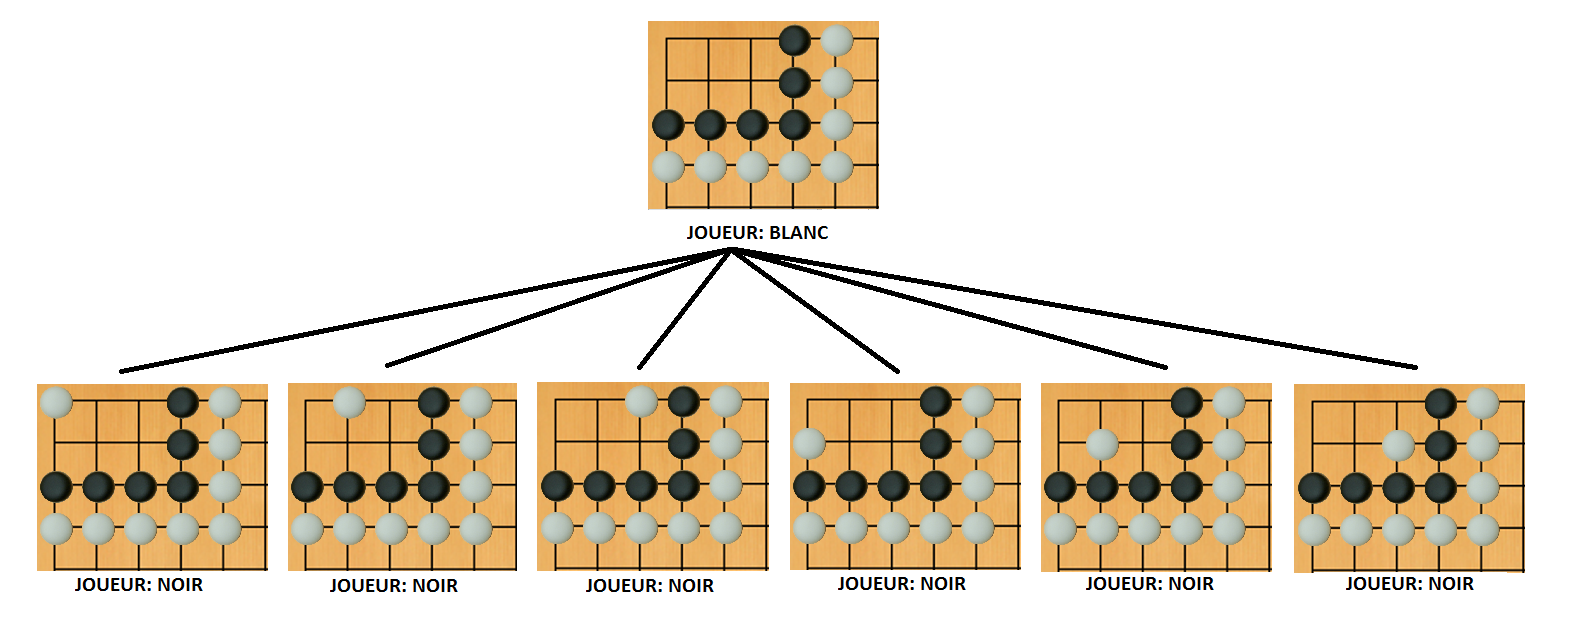
\includegraphics[scale=0.35]{figures/experiments/1.png}
        \caption{Les fils du premier n\oe ud dans le problème du 6 en coin}
        \label{fig:game}
        \end{figure}

        \paragraph{}Notre choix s’est arrêté sur une arborescence à n fils. Chaque nœuds de l’arborescence contient une valeur booléen dont le but est d’indiquer si ce nœud est gagnant.
        L'objet goban permet de connaître l’état de la partie à cet instant dans l’arbre. Chaque fils étant un état du jeu à l’instant T+1 (donc des gobans avec un coup supplémentaire). S’ajoute à cela une valeur, qui vaut blanc ou noir, afin de savoir qui doit jouer si on doit générer des fils à explorer ainsi qu'une variable renseignant le nombre de fils pour l'exploration.

            
    \section{Algorithmes}
        \subsection{Algorithme de définition des fils d'un noeud}
            Pour chaque noeud de l'arbre on calcule tout les coups possibles du joueur et pour chaque coup on crée un goban. On aura de cette manière les gobans des fils qui seront créés successivement à la base de ces premiers.\\
            Le nombre de gobans produit sera intuitivement le nombre d'états vides dans le goban de référence.
            
            \begin{framed}
                \underline{Voici les fonctions de l'algorithme :}
                \begin{itemize}
                    \item \textbf{jouer(Goban, VAL, x, y)}:
                    Soit un Goban et un État la fonction
                    contrôle si par rapport au règles du jeu on peut poser la pierre dans le goban.\\
                    Si la pierre peut être posée alors la placer et renvoyer vraie, sinon renvoyer faux.
                    
                    \item \textbf{rechercheGroupes(g)}:
                    Ajout de l'élément \textit{e} en queue du tableau \textit{t}.
                    
                    \item \textbf{itoc(i, goban)}:
                    Soit un entier et un goban \textit{i} il renvoie les coordonnées (x,y) de l'Etat pointé par \textit{i} dans le goban.
                \end{itemize}
            \end{framed}
            
            \begin{algorithme}
                \caption{définition des gobans fils}
                \textbf{Données :}
                \Type{goban}{Goban},
                \Type{value}{VAL};\\
                \textbf{Résultat :} renvoyer un tableau de gobans\\
                \textbf{Variables :}
                \Type{gob}{Goban},
                \Type{x}{entier},
                \Type{y}{entier},
                \Type{lisGob}{Goban[]},
                \textbf{Début :}\\
                \For{i \textbf{de} 0 \textbf{à} taille(goban)}
                {
                    x$\leftarrow$itoc(i, goban)[0]\\
                    y$\leftarrow$itoc(i, goban)[1]\\
                    gob$\leftarrow$goban\\
                    \If{jouer(gob, value, x, y)}
                    {
                        rechercheGroupes(gob)\\
                        EliminerGroupesAdversaire(value, gob)\\
                        ajoute(gob, listGob)
                    }
                }
                \textbf{renvoyer} listGob
            \end{algorithme}
            
        \subsection{Algorithme récursif du Tsumego}
            \paragraph{}L'algorithme du Tsumego et celui qui va résoudre le problème de vie ou de mort choisie par le joueur. Le principe est de vérifier si un groupe de pierre arrive à s'échapper (voir la partie problèmes plus bas).
            
            \paragraph{}La cible est représentée par une seule pierre appartenant au groupe ciblé. En effet, lorsqu'une pierre appartient à un groupe, celle-ci ne peut être prise si et seulement si le groupe entier est pris. Les données initiale du Tsumego seront donc une pierre, le goban -contenant le problème à résoudre-, l'état relatif à la cible et le joueur courant.
            
            \paragraph{}Si le premier joueur est de la même couleur que la cible alors son but sera de s'échapper. De la manière si le joueur est la couleur opposé il essayera de tuer la cible. 
            Ainsi si le premier joueur gagne alors l'information du noeud sera "vraie", autrement faux.
            
            \paragraph{}Les fils d'un noeud auront comme joueur adverse le joueur père, cela implique que si le fils renvoie l'information "vraie" cela signifiera ainsi qu'il aura survécu, et qu'il est alors nécessaire d'essayer un autre coup, ainsi si ce cas se répète le Tsumego parcourra tout les fils jusqu'à en trouver un qui lui renverra un faux qui signifie qu'il le joueur adverse n'aura pas survécu, donc que le groupe aura été capturé, rimant avec victoire, sinon il continuera à développé l'arbre.
            
            \begin{algorithme}
                \caption{Tsumego}
                \textbf{Données :}
                \Type{A}{Arbre},
                \Type{cible}{Etat};\\
                \textbf{Résultat :} développer \textit{A} pour résoudre le problème de vie ou de mort\\
                \textbf{Variables :}
                \Type{i}{entier},\\
                \textbf{Début :}\\
                \Rem{cas d'arrêt: A est une feuille}\
                \If{nbF(A) = 0}
                {
                    \IfThenElse{couleur(A) = couleur(cible) et enVie(cible,A) = vraie}
                    {
                        A.info = 1
                    }{
                        \IfThenElse{couleur(A)\neq couleur(cible) et enVie(cible,A) = faux}
                        {
                            A.info = 1
                        }{
                            A.info = 0
                        }
                    }
                    \textbf{renvoyer} ;
                }
                
                i$\leftarrow$0\\
                \While{i < nbF(A) et A.info = 0}
                {
                    \IfThenElse{A.joueur = BLANC}
                    {
                        val$\leftarrow$NOIR
                    }{
                        val$\leftarrow$BLANC
                    }
                    \Rem{creation de l'arbre fils}\\
                    A.filsA(GobansFils(A)[i], val)\\
                    \IfThenElse{enVie(cible,A.filsA)}
                    {
                        Tsumego(A.filsA, cible)
                    }{
                        [le coup a tué la cible et l'adversaire est le seul qui peut tuer]\\
                        A.info = 1\\
                        \textbf{renvoyer} ;
                    }
                    
                    \If{A.filsA.info = 0}
                    {
                        A.info = 1\\
                        \textbf{renvoyer} ;
                    }
                    i$\leftarrow$i + 1
                }
            \end{algorithme}
            
    
    
    
    \chapter{Optimisation \& Parseur}\label{chap:Optimisation}
    \section{Optimisation algorithmique}
        Nous avons utilisé deux types d'optimisation :
        \begin{itemize}
            \item La première est déjà implantée dans l'algo au-dessus, c'est ce qui distingue le tsumego brut, du tsumego normal. Elle se situe dans le while, c'est la condition A->Info == 0 ? : elle indique a l'algorithme de sortir de la boucle si on a tué le groupe, c'est ce qu'on appelle plus communément du \textbf{Pruning}.\\
            \item La deuxième a pour but de faire une économie mémoire dans notre tsumego, en effet au lieu de développer tout l'arbre des possibilités de coups possibles, ce qui ferait exploser la mémoire, nous développons qu'un "étage" de l'arbre, afin d'appliquer le tsumego sur chacun de ses éléments un à un en prenant bien soin d'effacer le fils précédent si la recherche développée à partir de celui-ci s'est révélée négative.
        \end{itemize}
            
    \section{Optimisation mémoire}
        \subsection{Format compression}
            \paragraph{}Afin d’essayer de résoudre des problèmes plus conséquents, nous nous somme penché sur l’optimisation mémoire pour la fonction de Tsumego. En analysant les instances présentes dans le Tsumego on se rends compte que ce sont les différentes instances de Goban qui sont coûteuses en mémoire. Nous avons cherché comment résoudre ceci et avons opté pour une paire de fonctions : une pour compresser le goban et une pour le décompresser.
    
            \paragraph{}Il a fallu pour cela définir un format économe pour stocker le Goban en mémoire et pour cela nous avons tenté d’éliminer les informations superflues. Tout d’abord nous avons fait le constat que seuls les états des intersections du goban étaient utiles pour reconstruire l’entièreté de celui-ci. En effet les différents groupes peuvent être retrouvés via la fonction de recherche de groupes, quant aux scores de chaque joueur et l’historique, ces informations ne sont d’aucune utilité pour le Tsumego. 
            
            \paragraph{}Ensuite nous avons cherché de la même manière à réduire l’espace mémoire de chaque intersection. Tout d’abord en éliminant les coordonnées de celles-ci car elles peuvent être trouvées automatiquement lors de la création d’un Goban. À ce Stade il ne nous restait plus qu’à trouver comment stocker les états. La façon la plus optimal étant de coder chaque état sur un nombre de bits défini puis de coller les états les uns à la suite des autres. 
            
            \paragraph{}De prime abord on pourrait penser qu’il nous faut coder jusqu’à 6 états différents (Blanc, Noir, Vide, KO\_blanc, KO\_noir, Non\_Jouable) cf. partie sur l’état d’une intersection de Goban. Par conséquent il nous faudrait 3 bits (6 < 8 = 2\^3) pour stocker n’importe quel état. Ors il se trouve que l’état Non\_Jouable n’a pas à être codé car il n’est pas stocké (pour les raisons évoqués ci-dessus). De plus les deux états de KO peuvent être résumer en un seul à condition de garder l’information sur le joueur courant à chaque étape du Tsumego. Il ne reste donc plus que 4 état possibles ce qui permet de coder n’importe quel état sur 2 bits seulement.
            
            \paragraph{}Grâce à ce format compressé un goban de 9 par 9 intersections peut être stocké sur 20 octets et 2 bits. Lorsque que l’on sait que son penchant non compressé pèse à minima 1ko (1040 octets pour être exact) à taille équivalente, on se rends compte de l’efficacité de la compression.
            \[ 9 * 9 = 81 intersections \,;\; 81 * 2 = 162 bits \,;\; 162 = 8 * 20 + 2\]
            Mais pour pouvoir stocker le Goban sous cette forme il faut écrire deux fonctions permettant de passer de la version compressée à celle de base et réciproquement.


        \newpage
        \subsection{Compression du Goban}
            \paragraph{}Pour la compression nous avons écrit l’algorithme qui suit. Cette version est assez bas niveau car nous parlons d’une compression binaire, néanmoins ce code a été simplifié pour faciliter sa compréhension. De même toutes les astuces pour économiser du temps de calcule sont passé sous silence. Nous espérons que le lecteur avisé ne s’offusquera pas de cet écart.
            
            \begin{algorithm}
                \caption{Algorithme de compression}
                \begin{algorithmic}
                %%-----------------------------------------------
                \REQUIRE goban : Goban à compresser (les cases inutiles sont marquées)
                \ENSURE Un tableau d'octets
        
                \STATE $nb\_rev \leftarrow \textit{nbInterUtiles}(goban);$
                \STATE $nb\_octets \leftarrow \textit{plafond}(\frac{nb\_rev}{8});$
                \STATE $nb\_bits\_bouchon \leftarrow 8 - (nb\_rev \mod 8);$
                \STATE $act \leftarrow 0;$
                \STATE $tmp \leftarrow 0;$
                \STATE $comp \leftarrow \textit{tableau}[nb\_octets]$
                
                \FORALL {$inter \in goban$}
                    \STATE $comp[cur] \leftarrow (comp[cur] << 2);$
                    \STATE $comp[cur] \leftarrow (comp[cur] + \textit{code}(inter));$
                    \IF{$tmp == 8$} 
                        \STATE $cur \leftarrow cur + 1;$
                        \STATE $tmp \leftarrow 0;$
                    \ENDIF
                \ENDFOR
         
                \STATE $comp[nb\_octets - 1] \leftarrow (comp[nb\_octets - 1] << nb\_bits\_bouchon);$
                \STATE \textbf{Retourner} $comp$.
                %%-----------------------------------------------
                \end{algorithmic}
            \end{algorithm}
    
            \begin{framed}
                    \underline{Notations :}
                    \begin{itemize}
                        \item A << N : décalage binaire N bits vers la gauche, appliqué à A ;
                        \item A >> N : décalage binaire N bits vers la droite, appliqué à A ;
                        \item Ob10101011 : représentation d’un octet en binaire non signé (dans cet exemple 171) ;
                        \item \& : le ET bit à bit de deux entiers sous leur forme binaire ;
                    \end{itemize}
                \end{framed}
    
    
        \subsection{Décompression du Goban}
            \paragraph{}Pour la décompression nous avons écrit l’algorithme qui suit. Cette version est assez bas niveau car nous parlons d’une compression binaire, néanmoins ce code a été simplifié pour faciliter sa compréhension. En particulier le cas du dernier octet compressé (celui pouvant contenir des bits de bourrage) a été omis pour éviter les doublons. Comme pour le cas de la compression, nous priions notre lecteur de ne pas s’offusquer de ces quelques imprécisions.
    
            \begin{algorithm}
                \caption{Algorithme de décompression}
                \begin{algorithmic}
                %%-----------------------------------------------
                \REQUIRE model : Goban où les case inutiles sont marquées, \\
                comp : tableau d'octet (goban compresssé)
                \ENSURE Goban décompressé
                
                \STATE $goban \leftarrow \textit{creerGoban}(model);$
                \STATE $nb\_rev \leftarrow \textit{nbInterUtiles}(goban);$
                \STATE $nb\_octets \leftarrow \textit{plafond}(\frac{nb\_rev}{8});$
                \STATE $nb\_bits\_bouchon \leftarrow 8 - (nb\_rev \mod 8);$
                \STATE $act \leftarrow -1;$
                \STATE $masque \leftarrow 0b11111100;$
                
                \FORALL {$i \in [0, nb\_octets]$}
                    \STATE $oct\_act \leftarrow comp[i];$
                    
                    \FORALL {$j \in [0, 4]$}
                        \STATE $val \leftarrow ((oct\_act \& masque) >> 6);$
                        \STATE $oct\_act \leftarrow oct\_act << 2;$
                        \STATE $act \leftarrow \textit{indiceProchaineItersectionUtile}(model);$
                        \STATE $goban[cur] \leftarrow tmp;$
                    \ENDFOR
                \ENDFOR
                
                \STATE \textbf{Retourner} $goban$.
                %%-----------------------------------------------
            \end{algorithmic}
            \end{algorithm}

            \begin{framed}
                    \underline{Notations :}
                    \begin{itemize}
                        \item A << N : décalage binaire N bits vers la gauche, appliqué à A ;
                        \item A >> N : décalage binaire N bits vers la droite, appliqué à A ;
                        \item Ob10101011 : représentation d’un octet en binaire non signé (dans cet exemple 171) ;
                        \item \& : le ET bit à bit de deux entiers sous leur forme binaire ;
                    \end{itemize}
                \end{framed}


    \section{Le parseur}
        \paragraph{}Afin d'implémenter plus facilement tout les problèmes les plus connus et complexes du Jeu de Go afin d'utiliser le Tsumego dessus, nous avons décidé de créer un parseur afin d'importer facilement les Goban nécessaires.
        
        \paragraph{}Nous avons défini une nouvelle extension .go, qui n'est au final qu'un fichier texte de quatre caractères différents :
        \begin{itemize}
            \item - " N " : Pour les pierres noires
            \item- " B " : Pour les pierres blanches
            \item- " - " : Pour les zones non jouables
            \item- " \_ ": Pour les zones vides jouables
        \end{itemize}
        
        \paragraph{}Puis on lit le fichier dans lequel chaque ligne correspond à une ligne du Goban pour remplir celui-ci petit à petit.

        \begin{algorithme}
            \caption{Parseur}
            \textbf{Données :}
            \Type{fichier}{String};\\
            \textbf{Résultat :} Rend un Goban parsé\\
            \textbf{Variables :}   
            \Type{goban}{Goban},
            \Type{y}{entier},
            \Type{x}{entier},
            \Type{piece}{char};\\
            \textbf{Début :}\\
            \IfThenElse{regex(".go",fichier)}
            {\textit{ouvrir} file(fichier);\\
            \IfThenElse{file}
                {x$\leftarrow$0\\
                y$\leftarrow$0\\
            \While{file.get(piece)}
                {\If{piece = 'B'}
                    {goban.coord(x , y).setVal(Blanc)}\\
                \If{piece = 'N' }
                    {goban.coord(x , y).setVal(Noir)}\\
                \If{piece = '-' }
                    {goban.coord(x , y).setVal(Vide)}\\
                \If{piece = '\_' }
                    {goban.coord(x , y).setVal(Non Jouable)}\\
                \If{piece = 'B' }
                    {goban.coord(x , y).setVal(Blanc)}\\
                \IfThenElse{piece = '/n' }{y++}
                {"Caractère lu inconnu à la position (" x ", " y ") !"}
                
                x < TGOBAN? x++ : x$\leftarrow$0\\}
            }
                {"Impossible d'ouvrir le fichier ! "}
            }{"Fichier introuvable"}
            \textbf{Renvoyer} goban
        \end{algorithme}
    \chapter{Conclusion}\label{chap:conclusion}
    \section{Bilan}
        \paragraph{}Nous sommes heureux d'annoncer que le Tsumego fonctionne pour le problème du 6 dans le coins, il détermine donc si le groupe va survivre ou pas. Du début jusqu'à la fin de ce projet les membres sont restés actifs ce qui nous à permis d'arriver à faire fonctionner notre algorithme de solution sur certains problèmes de Tsumego. C'est une réussite personnelle pour chaque membre car ce sujet de TER nous paraissait insurmontable en vu des échecs des précédentes années. Mais ce projet nous a intéressé et au delà du défi de réussir il nous a permis de nous enrichir autant techniquement que socialement. Au fur et à mesure du temps nous avons appris à nous connaître et à nous adapter avec le caractère des uns, parfois solitaire, et avec celui des autres. Et c'est ce que nous noterons de plus important lors d'un travail de groupe c'est de pouvoir s'adapter pour maintenir la cohésion.
            
    \section{Perspectives}
        \paragraph{}Nous aurions pu améliorer la performance du Tsumego en éliminant les gobans des fils. Ceci permettrait une économie de mémoire lors de l'appel récursif du tsumego. En effet nous n'aurions pas à recalculer l'intégralité des fils mais seulement ceux qui nous intéressent. 
        
        \paragraph{}De plus nous avions la possibilité d'utiliser le résultat du Tsumego pour créer une intelligence artificielle. Celle-ci aurait dû être capable de jouer contre une personne sur des problèmes de petite taille. Nous disposons de deux possibilités pour mettre en place cette IA. La première serait de lancer le Tsumego une seule fois puis d'utiliser l'arbre développé pour répondre aux coups du joueur. La seconde, plus économe en mémoire, serait l'utilisation d'une version alternative du Tsumego gardant en mémoire seulement le coup gagnant. Elle lancerait alors le Tsumego  après chaque coup du joueur.
        
        \paragraph{}Un tout autre cas de figure est aussi envisageable : ajouter à notre application une fonctionnalité de jeu en ligne. Cette possibilité permettrait de nous initier à la communication internet d'une application et serait un prolongement intéressant pédagogiquement parlant. De plus en poursuivant ce projet nous pourrions envisager de le publier en ligne et permettre à des amateurs de Go de jouer sur un logiciel libre et gratuit !

    \section{Apport personnels du projet}
        \paragraph{}Effectuer ce projet fut, pour chacun de nous, un gain en connaissances énorme. Il nous a permis d'en apprendre plus dans de nombreux domaines ainsi que de se perfectionner dans ceux que nous connaissions déjà. Cet apport ne s'est pas cantonné à l'informatique mais il a touché d'autre niveaux tels que la mise en page en Latex, dans le graphisme, la musique pour certains, la rédaction de rapport, etc. \\
        Au final les projets TER sont un apport considérable dans nos études. Ils nous mettent face à la réalité du travail en groupe et nous apporte de nombreuses compétences. C'est l'un des points fort de notre formation et cela fait même parfois émerger des vocations pour certains.

    \chapter{Remerciements}\label{chap:remerciements}
    \paragraph{}Nous tenons à remercier notre professeur référent pour ce TER : M. Pompidor qui a su se montrer présent pour nous tout au long de ce projet. Son soutient et ses précieux conseils nous ont été d’une aide précieuse.
    
    \paragraph{}Nous souhaiterions aussi remercier M. Dicky –enseignant d’algorithme au second semestre- pour les quelques astuces qu’il nous a fourni. La rigueur de son travail dans l’UE HLIN401 a été pour nous un exemple tout au long du projet.
    
    \paragraph{}Enfin nous remercions l’intégralité de nos enseignant(e)s qui de par leurs cours nous ont d’une certaine manière aidé dans ce projet.
    \chapter{Annexes}\label{chap:annexes}
    \section{Implémentation de la partie graphique}
        \paragraph{}Pour implémenter une fenêtre de jeu, il fallait répondre au problèmes suivant :\\
        Avoir un objet qui représente :
        
        \begin{itemize}
            \item une intersection dans un goban.
            \item un goban.
            \item les informations de la partie.
            \item la fenêtre de jeu.
        \end{itemize}
        
        \subsection{Le Jeu}
            \subsubsection{L'intersection}
                \paragraph{}Pour répondre à ce problème nous avons implémenter une classe nommée : "Square".\\
                Cette objet hérite de la classe SFML "drawable" afin d'être "dessinable". 
                Un objet square représente une intersection. Nous avons donc un couple de deux entiers pour les coordonnées (constante). Une valeur (Black, white ou None) pour savoir quoi afficher. 
                
    	        \paragraph{}Enfin en attribut de classe, en variable static, les sf::textures\^1 d'images à afficher (pierre noir ou blanche). \\
    	        On remarquera que les coordonnées n'apparaissent pas dans les attributs de la classe Square tout simplement car elles sont inutiles. En fait l'objet sf::sprite\^2 qui dessinera la pierre ou rien, contient déjà des coordonnées (relative à la fenêtre). \\
    	        De plus, pour la méthode "draw", qui est définis plus haut dans la hiérarchie (dans Drawable), sera virtuelle pour pouvoir être remplacée par celle définie dans Square.
    	        
    	   \subsubsection{Le Goban}
                \paragraph{}La classe Board, qui hérite aussi de drawable, représente un goban. Elle a donc comme attribut un objet Goban afin de manipuler toute les méthodes liées aux règles, à la recherche de groupes et à leurs manipulations.
                
    	        \paragraph{}Pour ce qui concerne l'affichage, nous aurons aussi en attribut un tableau d'objets "square" (qui sera dynamique). Une image, pour représenter graphiquement le goban. Un objet sf::view\^3 afin de pouvoir zoomer sur une partie du goban. 
    	        
    	        \paragraph{}Enfin, quatre variables pour les effets sonores, eux aussi présents dans la bibliothèque SFML.\\
                Un sf::SoundBuffer\^4 et un sf::Sound\^5 pour chaque son. Un lors de la pose d'une pierre, l'autre lors de la capture d'un groupe. 
                
                \paragraph{}Cet objet doit pouvoir interagir avec l'utilisateur. Poser des pierres dans le respect des règles du jeu. Pour se faire nous utilisons une méthode "click" qui vérifiera que le bouton pressé est bien le gauche grâce à la variable "event" de type "sf::Mouse::Button"\^6. Ensuite, on vérifie que les coordonnées du pointeur sont bien dans la zone de jeu et valide. Enfin on pose la pierre dans le goban en relançant la méthode de recherche de groupe pour mettre à jour les groupes. On joue un son lors de la pose, un autre si un groupe est éliminé. Enfin on applique la méthode load qui va convertir le goban en tableau de square afin de dessiner le nouveau goban.
                
            \subsubsection{Les Informations}
                \paragraph{}La classe infos nous permet d'afficher les informations sur la partie en cours : le joueur actuel (blanc ou noir) et le temps de jeu pris pour chaque joueur. 
                
    	        \paragraph{} Pour le temps nous utilisons une autre classe nommée "Timer" qui hérite des classes SFML, sf::Clock et sf::Text. Les attributs sont naturellement, un objet sf::Time, un "sf::Font" pour charger une police d'écriture et un booléen pour savoir si le temps est en "pause" ou non. Pour les mêmes raison que les objets square, lors de l'affichage du temps, on utilise un objet sf::Text qui à une position, une sf::Color\^7, une taille de caractère etc.. Il suffit donc de les définir lors de l'appel du constructeur.
    	
    	        
    	        \paragraph{} Nous dessinons donc chaque temps (blanc et noir) et à chaque changement de joueurs la méthode "pause()" est appelée. La méthode "setCurPlayer" permet en passant en paramètre la Square::Value (blanc ou noir) de savoir quel joueur doit jouer.
    	        
    	   \subsubsection{La fenêtre de Jeu}
                \paragraph{}La classe Game\_Window qui hérite de Screen, va avoir le rôle de chef d'orchestre lors du lancement d'une partie de Go. Elle a comme attribut une board, un infos et une value car a la valeur du joueur courant.
                
    	        \paragraph{}Quelques mots sur la classe "Screen". Elle hérite de "sf::Drawable". On y retrouve deux méthodes virtuelles publics : "draw", pour que tout ce qui hérite de "Screen" puisse redéfinir cette méthode (tout comme dans square). Et "Run", ce sera la méthode qui sera utiliser pour gérer les intersections et les évènements courants (un clique, un appuie sur un touche du clavier, etc..). Cette méthode retourne un "Screens". C'est une information afin de pouvoir gérer les différente fenêtre.
    	        
    	        \paragraph{}Dans Game\_Window nous retrouverons donc la méthode "Run", qui va s'occuper d'aiguiller les évènements à l'aide d'un "switch". Pour ce qui concerne le clique on va appeler la méthode "click". Elle fera un bref appel à la méthode "click" définie dans la classe board en transmettant les données, tel que la position et le joueur actuel qui sera modifiée lors de cette exécution. Bien évidemment, la méthode click de board étant un booléen, il sera utilisé pour le changement de tour du joueur (si le clique était autre chose que poser une pierre). Pour les évènements clavier on appel la fonction "keyPressed", qui en fonction de la touche exécutera une action, par exemple un "ctrl+Z" retire le coup qui vient d'être joué un "Escape" mets en pause le jeu et ouvre le menu de pause (nous expliquerons son fonctionnement plus tard).
        
        
        \subsection{Les menus}
            \paragraph{}Pour implémenter les menus nous avions besoin d'une image de fond et de plusieurs boutons afin de pouvoir naviguer parmi différentes fenêtres comme le jeu, les problèmes, les options...\\
            Pour y répondre nous avons créé deux classes. Une étant le menu "Menu" lui même et une autre gérant les boutons : "Choice".
            
            \subsubsection{Le Menu}
                \paragraph{}La classe "Menu" qui hérite de screen (vu précédemment) à pour attributs une sf::Texture qui sera la texture de l'arrière plan. Un sf::Sprite pour dessiner à l'aide de la méthode "draw" la texture. Enfin une variable de type Screens (énumération). On note aussi la présence de deux attributs accessibles par la classe et tout ses héritiers (protected), ce sont les objets "Choice" du menu, rassemblés dans un vecteur et un pointeur pour le Choice courant. Pour les méthodes, draw, Run, click auront les mêmes logiques que précédemment. 
                
    	        \paragraph{} Une méthode addItem est présente, elle prend en paramètre un objet Choice qui sera ajouté au vecteur. D'ailleurs la présence de std::reference\_wrapper" permet d'insérer les éléments par référence dans le "conteneur" ici le vecteur. 
    	       
    	   \subsubsection{Les Boutons}
                \paragraph{}La classe "Choice qui hérite de sf::Drawable aura comme attributs tout ce qui est nécessaire pour afficher un bouton (deux pointeurs sf::Texture et deux sf::Sprite). Pourquoi deux pointeurs sf::Texture ? Tout simplement car nous voulions afficher une image différente lors de la sélection d'un bouton (ici ce sera un léger liseré noir qui entourera le bouton). \\
                Pour savoir si ce dernier est sélectionné, nous avons un booléen "selected" pour renseigner cette information. 
                
    	        \paragraph{}Enfin, nous trouverons l'attribut sf::Text pour afficher le nom du bouton. Mais que fait ce bouton ? il y a un attribut "std::function<....". En fait c'est cette fonction (appelée lambda fonction) qui s'exécutera. Elle renvoi un entier, plus précisément un "Screens".
    
    	   \subsubsection{Les menus spéciaux}
                \paragraph{}Ces deux classes héritent de la classe "Menu". Ce choix particulier de créer deux autres classes de menus réponds à une vision des choses. Nous nous sommes posés la question : Vaut-il mieux instancier chaque images pour chaque boutons ou bien créer des menus avec des boutons identiques ? Pour nous, un menu affiche une ensemble de choix (les choices). Ces choix sont graphiquement identiques : même taille pour les boutons, une image et une sélection unique pour chaque bouton. \\
                Ayant le menu "Problème" qui devait contenir des choix graphiquement différents des autres menus nous avons donc créé une autre classe de menus. 
                
    	        \paragraph{}Leurs fonctionnements techniques sont identiques à ceux de leur père, menu. Cependant menu\_miniature est plus léger en termes de variables. Par exemple, il n'y a pas de "sf::Text" car chaque bouton affiche des images de problèmes à charger, l'utilité d'un texte était donc superflu. 
    	       
    	   \subsubsection{Les boutons spéciaux}
                \paragraph{}Ces deux classes héritent de Choice, comme nous l'avons expliqué pour la partie précédente le choice\_miniature (qui concerne le menu "problème") contiendra une référence de "sf::Texture" pour chaque image de problèmes à dessiner. L'autre classe, choice\_simple contiendra un sf::Text et un sf::Font en plus des attributs de la classe mère (même image pour tout les boutons).
        
        
        \subsection{Le Programme Principal}
            \subsubsection{}
                \paragraph{}Le programme principal (le main) doit gérer toutes les fenêtres de notre programme. On remarquera la présence d'une macro qui active le multi-threading. Nous nous intéresserons plus particulièrement à la fonction "renderingThread" qui va gérer les différents "screens" en fonction de ce que demande l'utilisateur. Ceci est géré grâce a un "while" qui vérifie que la fenêtre courante est différente de l'appel de fermeture. Toute les fenêtres seront présentes dans un "std::vector" d'objet "Screen" vu dans la partie I. Ajoutons que ces menus seront dessinés en effaçant la fenêtre courante à l'aide de la méthode ".clear" sur l'objet window qui est de type "sf::RenderWindow". Ensuite avec la méthode "draw" nous dessinerons la nouvelle fenêtre.
                
                \paragraph{}Pour plus de clarté nous avons séparé la gestion de ces menus avec leurs déclarations qui est décrite dans un objet "go\_solver". Cet objet contient donc comme attributs un "std::vector" de pointeur sur des screens, un "Screens" pour savoir quel est la fenêtre courante.\\
                Un "std::vector" pour la musique, si nous avons plusieurs piste par exemple. Une musique courante aussi. Une fenêtre de jeu spécifique à l'objet Game\_window" que nous avons vu qui sera appelée en cas de début de jeu. Enfin un "std::thread" pour le lancement du tsumego automatique afin de pouvoir interagir dans le programme pendant que le traitement s'effectue (qui peu être assez long).\\
                Cela permet entre autre, de fermer les programmes "proprement" à partir des boutons dédiés. \\
                La variable "target\_tsumego" permet de renseigner les informations concernant la cible à tuer (plus de précision sur la partie tsumego).
        
        \subsection{Glossaire}
            \begin{enumerate}
                \item Une texture est un objet qui réfère à une image.
                \item Une sprite est un objet qui est dessinable.
                \item Une view et une vue.
                \item SoundBuffer est un objet de la classe SFML.
                \item Sound aussi 
                \item Énumération dans SFML des évènement de souris.
                \item Ce type présent dans la SFML utilise une méthode qui n'a pas la même écriture sur Linux et sur Windows, d'où la présence d'une macro définissant setFillColor en setColor si nous somme sur Windows. 
            \end{enumerate}

    % La bibliographie n'est pas dans la table des matières par défaut, on l'ajoute donc manuellement. Ici on ne l'utilise pas.
    %\addcontentsline{toc}{chapter}{Bibliography}
    %\bibliographystyle{ieeetr}
    %\bibliography{bib/topic1,bib/topic2}
    %\newpage
    %\thispagestyle{empty}
    %\mbox{}
    

\end{document}
